%%%%%%%%%%%%%%%%%% Część II %%%%%%%%%%%%%%%%%

\section{Generowanie reguł decyzyjnych}

\subsection{Metoda pośrednia generowania reguł (\emph{C4.5rules})}
\begin{itemize}
\item \textbf{Wygeneruj reguły dla zbioru \emph{GOLF} za~pomocą programu \emph{C4.5 for Windows}.}

\begin{figure}
\begin{verbatim}
Rule 1: [70.7%]
    IF    outlook = overcast
    THEN  Play

Rule 2: [63.0%]
    IF    outlook = rain
    AND   windy = false
    THEN  Play

Rule 3: [63.0%]
    IF    outlook = sunny
    AND   humidity > 75
    THEN  Don't Play

Rule 4: [50.0%]
    IF    outlook = rain
    AND   windy = true
    THEN  Don't Play

Default class: Play

Errors in training set: 0 (0.0%)
\end{verbatim}
\caption{Reguły decyzyjne dla zbioru \emph{golf} uzyskane algorytmem \emph{C4.5rules}}
\label{p2t1-rules}
\end{figure}

	\\Wyniki pokazane są na Rys.~\ref{p2t1-rules}.

\item \textbf{Porównaj wygenerowane reguły z~wyjściowym drzewem decyzyjnym. Czy reguły odzwierciedlają precyzyjnie drzewo?}

\begin{figure}
	\begin{verbatim}
	
	Pruned decision tree:
	
	outlook = overcast: Play (4.0/1.2)
	outlook = sunny:
	|   humidity <= 75 : Play (2.0/1.0)
	|   humidity > 75 : Don't Play (3.0/1.1)
	outlook = rain:
	|   windy = true: Don't Play (2.0/1.0)
	|   windy = false: Play (3.0/1.1)

	\end{verbatim}
	
	\caption{Drzewo decyzyjne dla zbioru \emph{golf} uzyskane algorytmem \emph{C4.5}}

	\label{p2t1-tree}

\end{figure}


	\\Wyjściowe drzewo zostało przedstawione na Rys.~\ref{p2t1-tree}. Drzewo to nie może być odtworzone przy użyciu samych tylko uzyskanych reguł (Rys.~\ref{p2t1-rules}). Jest tak, ponieważ nie pokrywają one wszystkich możliwych ścieżek od~korzenia do liścia -- brakuje reguły dla \texttt{outlook = sunny AND humidity <= 75}. Ponieważ jednak w~wyniku zawarta jest również klasa domyślna, w~tym wypadku \texttt{Play}, możemy ją wykorzystać jako liść dla ścieżek w~drzewie odpowiadającym brakującym regułom. W~ten sposób, w~tym konkretnym przypadku, możliwe jest zrekonstruowanie drzewa. Stąd reguły odzwierciedlają drzewo w~sposób precyzyjny.
\end{itemize}

\subsection{Porównanie klasyfikowania za pomocą drzew decyzyjnych i~reguł decyzyjnych (\emph{C4.5rules})}
\begin{itemize}
\item \textbf{Przeprowadź testy \emph{10-fold CV} na wybranych zbiorach dla drzew i~reguł.}

\begin{table}
\begin{tabular}{|r||r|rr|rr||r|rr|rr|r|}
\hline
&\multicolumn{5}{c||}{Before pruning}&\multicolumn{6}{|c|}{After pruning} \\
\hline
Tree & 
Size & 
\multicolumn{2}{|c|}{Errors} & 
\multicolumn{2}{c||}{Errors (test)} & 
Size & 
\multicolumn{2}{|c|}{Errors} & 
\multicolumn{2}{|c|}{Errors (test)} & 
Estimate \\
\hline\hline
    1 &    8 &    0 &  0.0\% &    0 &   0.0\% &    8 &    0 &  0.0\% &    0 &   0.0\% &  43.5\%  \\
    2 &    8 &    0 &  0.0\% &    1 &  50.0\% &    8 &    0 &  0.0\% &    1 &  50.0\% &  43.1\%  \\
    3 &    6 &    2 & 16.7\% &    1 &  50.0\% &    1 &    4 & 33.3\% &    1 &  50.0\% &  47.5\%  \\
    4 &    6 &    1 &  8.3\% &    1 &  50.0\% &    6 &    1 &  8.3\% &    1 &  50.0\% &  44.5\%  \\
    5 &    6 &    1 &  7.7\% &    1 & 100.0\% &    6 &    1 &  7.7\% &    1 & 100.0\% &  42.1\%  \\
    6 &    8 &    0 &  0.0\% &    0 &   0.0\% &    8 &    0 &  0.0\% &    0 &   0.0\% &  41.0\%  \\
    7 &    8 &    0 &  0.0\% &    0 &   0.0\% &    8 &    0 &  0.0\% &    0 &   0.0\% &  41.0\%  \\
    8 &    8 &    0 &  0.0\% &    0 &   0.0\% &    8 &    0 &  0.0\% &    0 &   0.0\% &  40.6\%  \\
    9 &    8 &    0 &  0.0\% &    0 &   0.0\% &    8 &    0 &  0.0\% &    0 &   0.0\% &  40.6\%  \\
   10 &    6 &    1 &  7.7\% &    1 & 100.0\% &    6 &    1 &  7.7\% &    1 & 100.0\% &  42.1\%  \\
\hline\hline
 Avg. &  7.2 &  0.5 &  4.0\% &  0.5 &  35.0\% &  6.7 &  0.7 &  5.7\% &  0.5 &  35.0\% &  42.6\%  \\
\hline
\end{tabular}
\caption{\emph{Cross-validation} dla drzew utworzonych ze zbioru \emph{golf}}
\label{p2t2-golf-trees-cv}
\end{table}

\begin{table}
\begin{tabular}{|r|r|rr|rr|}
\hline
 Ruleset & 
 Size & 
 \multicolumn{2}{1|}{Errors} & 
 \multicolumn{2}{1|}{Errors (test)} \\
\hline\hline
       1 &    2 &    0 &  0.0\%  &    0 &   0.0\% \\
       2 &    3 &    0 &  0.0\%  &    1 &  50.0\% \\
       3 &    1 &    4 & 33.3\%  &    1 &  50.0\% \\
       4 &    3 &    1 &  8.3\%  &    2 & 100.0\% \\
       5 &    4 &    1 &  7.7\%  &    1 & 100.0\% \\
       6 &    4 &    0 &  0.0\%  &    0 &   0.0\% \\
       7 &    4 &    0 &  0.0\%  &    0 &   0.0\% \\
       8 &    3 &    0 &  0.0\%  &    0 &   0.0\% \\
       9 &    3 &    0 &  0.0\%  &    0 &   0.0\% \\
      10 &    2 &    1 &  7.7\%  &    1 & 100.0\% \\
\hline\hline
    Avg. &  2.9 &  0.7 &  5.7\%  &  0.6 &  40.0\% \\
\hline
\end{tabular}
\caption{\emph{Cross-validation} dla reguł utworzonych ze zbioru \emph{golf}}
\label{p2t2-golf-rules-cv}
\end{table}

\begin{table}
\begin{tabular}{|r||r|rr|rr||r|rr|rr|r|}
\hline
&\multicolumn{5}{1||}{Before pruning}&\multicolumn{6}{1|}{After pruning} \\
\hline
Tree & 
Size & 
\multicolumn{2}{1|}{Errors} & 
\multicolumn{2}{1||}{Errors (test)} & 
Size & 
\multicolumn{2}{1|}{Errors} & 
\multicolumn{2}{1|}{Errors (test)} & 
Estimate \\
\hline\hline
    1 &   25 &    7 & 2.6\% &    4 & 13.3\% &    7 &   12 & 4.4\% &    1 &  3.3\%  &   7.3\%  \\
    2 &   25 &    7 & 2.6\% &    1 &  3.3\% &    7 &   12 & 4.4\% &    1 &  3.3\%  &   7.2\%  \\
    3 &   16 &    9 & 3.3\% &    0 &  0.0\% &    7 &   13 & 4.8\% &    0 &  0.0\%  &   7.7\%  \\
    4 &   19 &   10 & 3.7\% &    1 &  3.3\% &    7 &   13 & 4.8\% &    0 &  0.0\%  &   7.7\%  \\
    5 &   16 &    8 & 3.0\% &    1 &  3.3\% &    7 &   11 & 4.1\% &    2 &  6.7\%  &   6.9\%  \\
    6 &   16 &    8 & 3.0\% &    4 & 13.3\% &    7 &   11 & 4.1\% &    2 &  6.7\%  &   6.9\%  \\
    7 &   31 &    5 & 1.9\% &    4 & 13.3\% &    4 &   13 & 4.8\% &    2 &  6.7\%  &   7.0\%  \\
    8 &   28 &    5 & 1.9\% &    4 & 13.3\% &    4 &   12 & 4.4\% &    3 & 10.0\%  &   6.6\%  \\
    9 &   16 &    7 & 2.6\% &    2 &  6.7\% &    7 &   11 & 4.1\% &    2 &  6.7\%  &   6.8\%  \\
   10 &   13 &    8 & 3.0\% &    3 & 10.0\% &    7 &   11 & 4.1\% &    2 &  6.7\%  &   6.8\%  \\
\hline\hline
 Avg. & 20.5 &  7.4 & 2.8\% &  2.4 & 8.0\%  &  6.4 & 11.9 & 4.4\% &  1.5 &  5.0\%  &   7.1\%  \\
\hline
\end{tabular}
\caption{\emph{Cross-validation} dla drzew utworzonych ze zbioru \emph{vote}}
\label{p2t2-vote-trees-cv}
\end{table}

\begin{table}
\begin{tabular}{|r|r|rr|rr|}
\hline
 Ruleset & 
 Size & 
 \multicolumn{2}{1|}{Errors} & 
 \multicolumn{2}{1|}{Errors (test)} \\
\hline\hline
       1 &    4 &   12 & 4.4\% &    1 &  3.3\% \\
       2 &    3 &   12 & 4.4\% &    1 &  3.3\% \\
       3 &    5 &   11 & 4.1\% &    0 &  0.0\% \\
       4 &    4 &   13 & 4.8\% &    0 &  0.0\% \\
       5 &    5 &    9 & 3.3\% &    2 &  6.7\% \\
       6 &    4 &   11 & 4.1\% &    2 &  6.7\% \\
       7 &    4 &    7 & 2.6\% &    2 &  6.7\% \\
       8 &    4 &    9 & 3.3\% &    4 & 13.3\% \\
       9 &    4 &    9 & 3.3\% &    2 &  6.7\% \\
      10 &    5 &    8 & 3.0\% &    3 & 10.0\% \\
\hline\hline
    Avg. &  4.2 & 10.1 & 3.7\% &  1.7 &  5.7\% \\
\hline
\end{tabular}
\caption{\emph{Cross-validation} dla reguł utworzonych ze zbioru \emph{vote}}
\label{p2t2-vote-rules-cv}
\end{table}

	\\Wyniki uzyskane z~programu \emph{C4.5 for windows} zostały przedstawione następująco: dla zbioru \emph{golf} w~Tab.~\ref{p2t2-golf-trees-cv} oraz Tab.~\ref{p2t2-golf-rules-cv}, dla zbioru \emph{vote} w~Tab.~\ref{p2t2-vote-trees-cv} oraz Tab.~\ref{p2t2-vote-rules-cv}.

\item \textbf{Porównaj wyniki pod kątem trafności klasyfikowania na zbiorze testującym oraz rozmiaru opisu.}
	
	\begin{figure}
	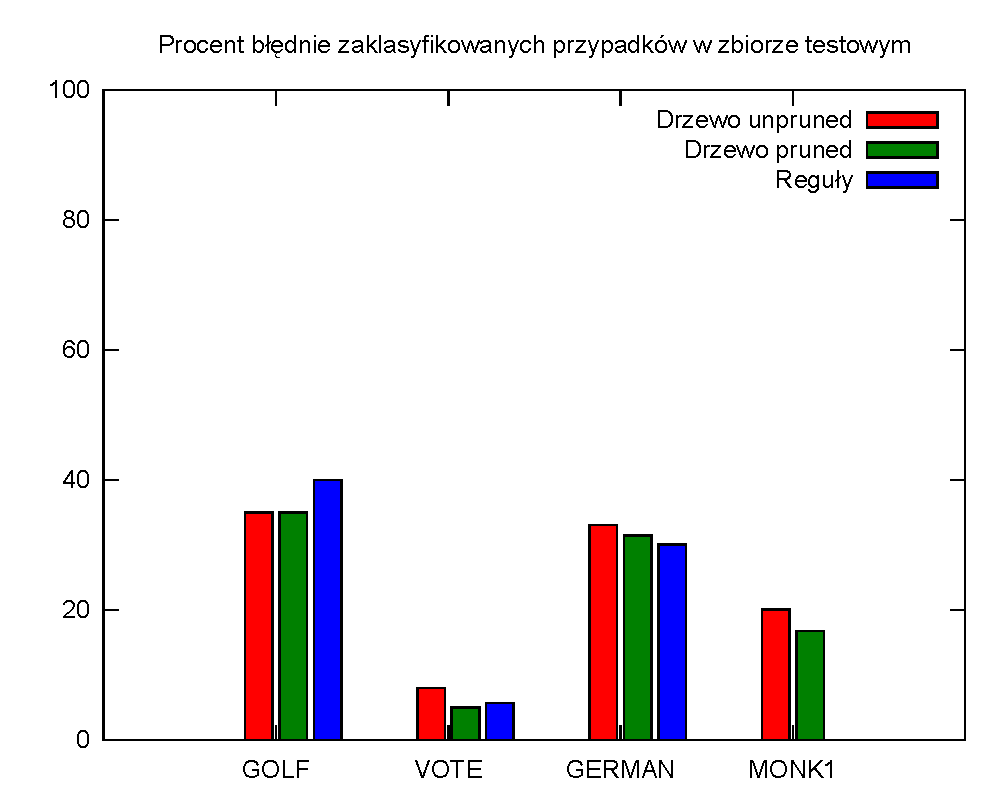
\includegraphics[scale=0.7]{gnuplot/compare-errors.pdf} 
	\caption{Błędy klasyfikowania na zbiorze testującym.}
	\label{p2t2-compare-errors}
\end{figure}

	\\Na Rys.~\ref{p2t2-compare-errors} przedstawiono zależność między trafnością klasyfikowania a~typem reprezentacji (drzewa, reguły). Dla wszystkich zbiorów danych z~wyjątkiem \emph{golf} reprezentacja regułowa daje lepszą klasyfikację niż drzewa. (Drobne różnice między drzewem po pruningu a~regułami dla zbioru \emph{vote} pomijamy.)
	\\Odmienną zależność dla zbioru \emph{golf} możemy tłumaczyć małą liczbą przypadków uczących w~tym zbiorze -- zaledwie 14~przykładów -- przez co zbiory testowe zawierają 1-2~przypadków testowych. W~tej sytuacji pojedynczy błąd ma istotny wpływ na końcową jakość klasyfikacji.
	
	\begin{figure}
	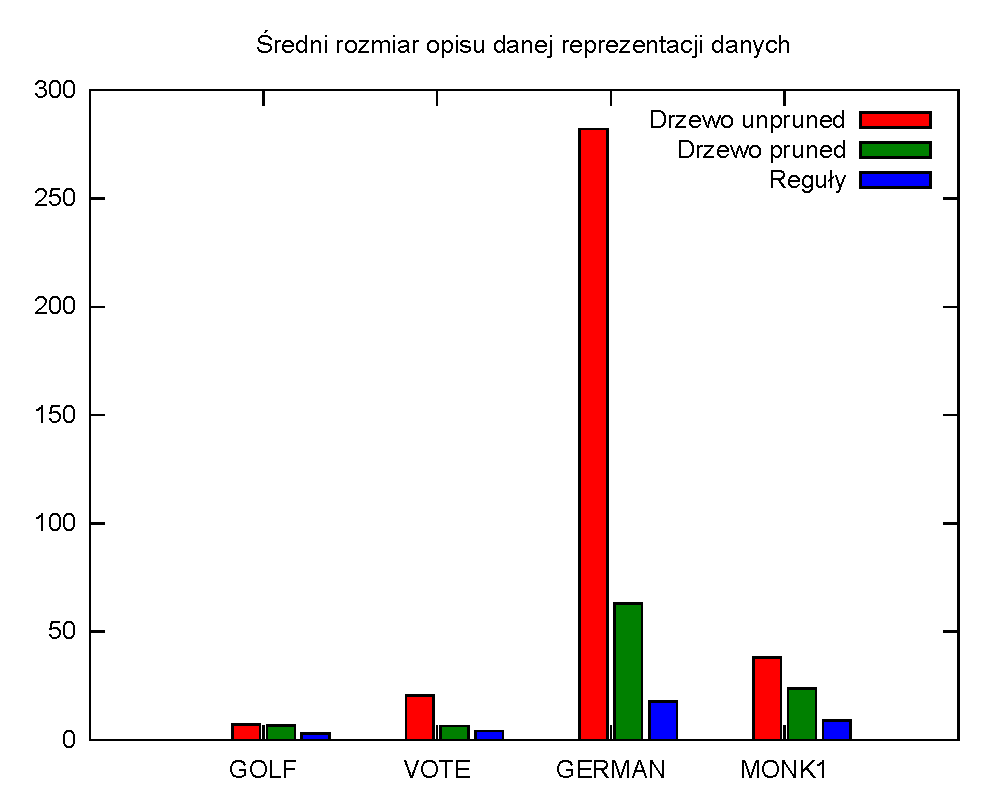
\includegraphics[scale=0.7]{gnuplot/compare-sizes.pdf} 
	\caption{Rozmiar opisu różnych reprezentacji wiedzy.}
	\label{p2t2-compare-sizes}
\end{figure}

	\\Na Rys.~\ref{p2t2-compare-sizes} dokonano porównania rozmiarów różnych reprezentacji wiedzy dla kilku wybranych zbiorów danych. Jako jednostkę przyjęto w~przypadku drzew pojedynczy liść, zaś w~przypadku reguł pojedynczą regułę. Widać znaczną redukcję rozmiaru przy przejściu od drzew bez pruningu przez drzewa z~pruningiem do reguł.
	
\item \textbf{Przeprowadzając kilka eksperymentów uczenia i~testowania przeanalizuj wpływ parametrów \emph{Confidence Level} i~\emph{Redundancy Factor} na~otrzymywany zbiór reguł.}

	\begin{table}
\begin{tabular}{|r|r|rr|rr|}
\hline
 Confidence Level & 
 Avg. Size & 
 \multicolumn{2}{|c|}{Avg. Errors} & 
 \multicolumn{2}{|c|}{Avg. Errors (test)} \\
\hline\hline
      0.10 &    2.9 &   11.4 & 4.2\% &    1.8 &  6.0\% \\
      0.30 &    4.2 &   10.0 & 3.7\% &    1.8 &  6.0\% \\
      0.50 &    4.8 &    9.1 & 3.4\% &    1.8 &  6.0\% \\
      0.60 &    5.2 &    8.8 & 3.2\% &    1.8 &  6.0\% \\      
      0.75 &    7.3 &    8.2 & 3.0\% &    1.8 &  6.0\% \\
      1.00 &    7.9 &    8.2 & 3.0\% &    1.8 &  6.0\% \\
\hline
\end{tabular}
\caption{Wpływ parametru \emph{Confidence Level} na~rozmiar zbioru reguł wygenerowanego dla zbioru \emph{vote}}
\label{p2t2-vote-confidence-level}
\end{table}

	\\Parametr \emph{Confidence Level} steruje liczbą i~rozmiarem reguł. Dla zbioru \emph{vote} zależność między wartością tego parametru a~rozmiarem zbioru reguł i~liczbą błędów przy klasyfikacji przedstawia tabela \ref{p2t2-vote-confidence-level}. Jak widać, zwiększenie wartości parametru prowadzi do zwiększenia rozmiaru zbioru reguł. Wprawdzie oznacza to polepszenie klasyfikacji dla zbioru uczącego, jednak (w~przypadku zbioru \emph{vote}) nie zauważono wpływu na jakość klasyfikacji dla zbioru testowego.

	\begin{table}
\begin{tabular}{|r|r|rr|rr|}
\hline
 Redundancy Factor & 
 Avg. Size & 
 \multicolumn{2}{|c|}{Avg. Errors} & 
 \multicolumn{2}{|c|}{Avg. Errors (test)} \\
\hline\hline
      0.10 &    2.0 &    13.5 & 5.0\% &    1.5 &  5.0\% \\
      0.30 &    2.0 &    13.5 & 5.0\% &    1.5 &  5.0\% \\
      0.40 &    3.0 &    11.3 & 4.2\% &    1.7 &  5.7\% \\
      0.50 &    3.5 &    11.3 & 4.2\% &    1.7 &  5.7\% \\
      0.75 &    4.4 &     9.7 & 3.6\% &    1.8 &  6.0\% \\
      1.00 &    4.8 &     9.1 & 3.4\% &    1.8 &  6.0\% \\
\hline
\end{tabular}
\caption{Wpływ parametru \emph{Redundancy Factor} na~rozmiar zbioru reguł wygenerowanego dla zbioru \emph{vote}}
\label{p2t2-vote-redundancy-factor}
\end{table}

	\\Parametr \emph{Redundancy Factor} steruje wyborem atrybutów do~reguł. Dla zbioru \emph{vote} zależność między wartością parametru a~rozmiarem zbioru reguł i~liczbą błędów przy klasyfikacji przedstawiona jest w~tabeli \ref{p2t2-vote-redundancy-factor}. Im mniejsza wartość parametru, tym mniej atrybutów zostanie wybranych do pojedynczej reguły decyzyjnej, co wpływa bezpośrednio na rozmiar samego zbioru reguł. W~zbiorze \emph{vote} zaobserwowano polepszenie klasyfikacji dla małych wartości \emph{Redundancy Factor}.

	\\Podsumowując, sterując tymi parametrami można uniknąć przeuczenia systemu, efekty jednak zależeć będą od~konkretnego zbioru przykładów uczących.
\end{itemize}


	\subsection{Generowanie reguł z~użyciem algorytmu \emph{LEM}}

\begin{itemize}
\item \textbf{Wygeneruj reguły dla zbioru \emph{HPAP.ISF}.}

	\begin{figure}
\begin{verbatim}
rule 1.
(Hem = f) & (Temp = l) => (Comfort = l);
[2, 2, 66.67%, 100.00%][2, 0, 0]
[{1, 2}, {}, {}]

rule 2.
(Temp = l) & (Hem = g) => (Comfort = m);
[2, 2, 50.00%, 100.00%][0, 2, 0]
[{}, {5, 6}, {}]

rule 3.
(Blood = n) & (Temp = n) => (Comfort = m);
[1, 1, 25.00%, 100.00%][0, 1, 0]
[{}, {7}, {}]

rule 4.
(Blood = h) => (Comfort = vl);
[2, 2, 100.00%, 100.00%][0, 0, 2]
[{}, {}, {8, 9}]

! Approximate rules
rule 5.
(Blood = l) & (Temp = n) => (Comfort = l) OR (Comfort = m);
[2, 2, 100.00%, 100.00%][1, 1, 0]
[{3}, {4}, {}]
\end{verbatim}
\caption{Reguły decyzyjne dla zbioru \emph{hpap} uzyskane algorytmem \emph{LEM}}
\label{p2t2-hpap-rules}
\end{figure}

	\\Wygenerowane reguły zostały przedstawione na rysunku \ref{p2t2-hpap-rules}.

\item \textbf{Przyjrzyj się regułom możliwym; opisz je i~,,wydedukuj'', skąd się wzięły.}
\end{itemize}

	\\Reguły 1--4 to reguły pewne, natomiast reguła 5~jest regułą przybliżoną. Reguła 1~pokrywa 2~z~3 obiektów klasy $l$, stąd jej pokrycie wynosi 66\%, reguła 2~pokrywa dwa obiekty z~klasy $m$ (pokrycie 50\%), reguła 3~pokrywa jeden obiekt z klasy $m$ (pokrycie 25\%), natomiast reguła 4~pokrywa oba obiekty z~klasy $v1$. Pozostały dwa obiekty nie pokryte przez żadną regułę pewną -- wynika to z faktu, że mimo iż posiadają identyczne wartości atrybutów, należą do dwóch różnych klas. Stąd reguła~5, przybliżona, która przypisuje obiekty jednocześnie do dwóch klas. Gdyby chcieć zamienić ją na reguły możliwe, należy usunąć jedną z~klas umieszczonych w~alternatywie.

\subsection{Porównanie reguł generowanych za~pomocą algorytmu \emph{LEM} i~\emph{C4.5}}

\begin{itemize}
\item \textbf{Wygeneruj reguły przy użyciu obu podejść dla zbiorów: \emph{HPAP}, \emph{VOTE} i~\emph{MONK}.}

	\begin{figure}
\begin{verbatim}
Rule 1: [50.0%]
    IF    blood = h
    THEN  vl

Default class: m

Errors in training set: 3 (33.3%)
\end{verbatim}
\caption{Reguły decyzyjne dla zbioru \emph{hpap} uzyskane algorytmem \emph{C4.5-rules}}
\label{p2t2-hpap-rules-c45}
\end{figure}

	\begin{figure}
\begin{verbatim}
rule 1. (A9 = n) & (A3 = n) & (A7 = n) & (A12 = y) & (A11 = n) => (A17 = republican)
rule 2. (A13 = y) & (A3 = n) & (A1 = n) & (A12 = y) & (A11 = y) &
        (A2 = y) => (A17 = republican)
rule 3. (A4 = y) & (A2 = n) & (A10 = y) => (A17 = republican)
rule 4. (A9 = n) & (A13 = y) & (A3 = n) & (A2 = y) & (A11 = n) => (A17 = republican)
rule 5. (A3 = n) & (A8 = ?) => (A17 = republican)
rule 6. (A4 = y) & (A6 = y) & (A15 = n) & (A16 = y) => (A17 = republican)
rule 7. (A4 = y) & (A9 = n) & (A7 = y) => (A17 = republican)
rule 8. (A14 = y) & (A12 = ?) & (A1 = n) => (A17 = republican)
rule 9. (A4 = y) & (A1 = y) & (A16 = n) & (A3 = n) => (A17 = republican)
rule 10. (A5 = ?) & (A9 = ?) => (A17 = republican)
rule 11. (A4 = ?) & (A16 = ?) & (A14 = n) => (A17 = republican)
rule 12. (A4 = y) & (A5 = n) & (A10 = y) => (A17 = republican)
rule 13. (A4 = n) & (A3 = y) => (A17 = democrat)
rule 14. (A11 = y) & (A2 = n) & (A16 = n) & (A1 = n) => (A17 = democrat)
rule 15. (A13 = y) & (A16 = ?) & (A1 = y) => (A17 = democrat)
rule 16. (A16 = n) & (A13 = n) => (A17 = democrat)
rule 17. (A12 = y) & (A4 = n) => (A17 = democrat)
rule 18. (A12 = n) & (A7 = y) & (A2 = ?) => (A17 = democrat)
rule 19. (A16 = y) & (A4 = ?) => (A17 = democrat)
rule 20. (A15 = n) & (A4 = n) => (A17 = democrat)
rule 21. (A13 = y) & (A3 = y) & (A16 = ?) => (A17 = democrat)
rule 22. (A3 = n) & (A15 = y) & (A2 = y) => (A17 = democrat)
rule 23. (A9 = y) & (A3 = n) & (A1 = y) => (A17 = democrat)
rule 24. (A12 = ?) & (A9 = y) => (A17 = democrat)
rule 25. (A11 = y) & (A13 = y) & (A10 = y) & (A12 = n) => (A17 = democrat)
\end{verbatim}
\caption{Reguły decyzyjne dla zbioru \emph{vote} uzyskane algorytmem \emph{LEM}}
\label{p2t2-vote-rules}
\end{figure}

	\begin{figure}
\begin{verbatim}
Rule 1: [98.4%]
    IF    physician fee freeze = n
    THEN  democrat

Rule 2: [97.5%]
    IF    synfuels corporation cutback = y
    AND   duty free exports = y
    THEN  democrat

Rule 3: [63.0%]
    IF    physician fee freeze = u
    AND   mx missile = n
    THEN  democrat

Rule 4: [88.7%]
    IF    physician fee freeze = y
    THEN  republican

Rule 5: [50.0%]
    IF    physician fee freeze = u
    AND   mx missile = u
    THEN  republican

Default class: democrat

Errors in training set: 11 (3.7%)
Errors in test     set: 6 (4.4%)
\end{verbatim}
\caption{Reguły decyzyjne dla zbioru \emph{vote} uzyskane algorytmem \emph{C4.5-rules}}
\label{p2t2-vote-rules-c45}
\end{figure}

	\begin{figure}
\begin{verbatim}
rule 1. (a1 = 1) & (a2 = 3) & (a5 = 3) => (d = 0)
rule 2. (a5 = 2) & (a2 = 1) & (a1 = 3) => (d = 0)
rule 3. (a5 = 4) & (a2 = 2) & (a1 = 1) => (d = 0)
rule 4. (a3 = 2) & (a1 = 2) & (a2 = 1) => (d = 0)
rule 5. (a1 = 2) & (a4 = 2) & (a5 = 4) => (d = 0)
rule 6. (a5 = 3) & (a1 = 2) & (a2 = 1) => (d = 0)
rule 7. (a2 = 3) & (a1 = 1) & (a5 = 4) => (d = 0)
rule 8. (a2 = 2) & (a1 = 1) & (a5 = 3) => (d = 0)
rule 9. (a2 = 3) & (a5 = 3) & (a1 = 2) => (d = 0)
rule 10. (a5 = 2) & (a1 = 1) & (a2 = 3) => (d = 0)
rule 11. (a2 = 2) & (a1 = 3) & (a5 = 4) => (d = 0)
rule 12. (a5 = 2) & (a6 = 1) & (a2 = 2) & (a4 = 3) => (d = 0)
rule 13. (a5 = 4) & (a4 = 3) & (a2 = 1) => (d = 0)
rule 14. (a5 = 3) & (a1 = 3) & (a2 = 1) => (d = 0)
rule 15. (a5 = 2) & (a1 = 2) & (a2 = 1) => (d = 0)
rule 16. (a5 = 2) & (a1 = 2) & (a2 = 3) => (d = 0)
rule 17. (a2 = 2) & (a5 = 3) & (a1 = 3) => (d = 0)
rule 18. (a5 = 2) & (a2 = 2) & (a1 = 1) => (d = 0)
rule 19. (a5 = 4) & (a1 = 2) & (a2 = 3) => (d = 0)
rule 20. (a1 = 2) & (a2 = 2) => (d = 1)
rule 22. (a1 = 3) & (a2 = 3) => (d = 1)
rule 23. (a2 = 1) & (a1 = 1) => (d = 1)
\end{verbatim}
\caption{Reguły decyzyjne dla zbioru \emph{monk1} uzyskane algorytmem \emph{LEM}}
\label{p2t2-monk-rules}
\end{figure}

	\begin{figure}
\begin{verbatim}
Rule 1: [95.3%]
    IF    attribute#5 = 1
    THEN  1

Rule 2: [92.2%]
    IF    attribute#1 = 3 AND   attribute#2 = 3
    THEN  1

Rule 3: [91.2%]
    IF    attribute#1 = 2 AND   attribute#2 = 2
    THEN  1

Rule 4: [85.7%]
    IF    attribute#1 = 1 AND   attribute#2 = 1
    THEN  1

Rule 5: [84.1%]
    IF    attribute#1 = 1 AND   attribute#2 = 3 AND   attribute#5 = 4
    THEN  0

Rule 6: [79.4%]
    IF    attribute#1 = 1 AND   attribute#2 = 3 AND   attribute#5 = 2
    THEN  0

Rule 7: [79.4%]
    IF    attribute#1 = 2 AND   attribute#2 = 1 AND   attribute#5 = 4
    THEN  0

Rule 8: [78.4%]
    IF    attribute#1 = 1 AND   attribute#2 = 2
    THEN  0

Rule 9: [66.2%]
    IF    attribute#4 = 2 AND   attribute#5 = 2
    THEN  0

Rule 10: [63.8%]
    IF    attribute#5 = 3 AND   attribute#6 = 1
    THEN  0

Rule 11: [63.5%]
    IF    attribute#3 = 2 AND   attribute#5 = 2
    THEN  0

Rule 12: [58.7%]
    IF    attribute#3 = 2 AND   attribute#5 = 3
    THEN  0

Default class: 0

Errors in training set: 0 (0.0%)
Errors in test     set: 0 (0.0%)
\end{verbatim}
\caption{Reguły decyzyjne dla zbioru \emph{monk1} uzyskane algorytmem \emph{C4.5-rules}}
\label{p2t2-monk-rules-c45}
\end{figure}

\item Przyjrzyj się niezależnie regułom pewnym i~możliwym (\emph{LEM}).
\end{itemize}

%Dla chętnych:
%\subsection{Przeprowadź eksperyment generowania i~testowania reguł LEM w~ramach cross validation}